\chapter{Réalisation}

\section{Introduction}

Ce chapitre présente la réalisation concrète de LudoHeritage. Après avoir décrit l'environnement
de développement et les technologies utilisées, nous parcourons les principales fonctionnalités
de l'application à travers des captures d'écran et des explications techniques ciblées.

% ─────────────────────────────────────────────────────────────────────────────
\section{Environnement de développement}
% ─────────────────────────────────────────────────────────────────────────────

\begin{table}[H]
\centering
\renewcommand{\arraystretch}{1.4}
\begin{tabularx}{\textwidth}{>{\bfseries}p{4cm} X}
\toprule
\textbf{Outil / Technologie} & \textbf{Rôle dans le projet} \\
\midrule
IntelliJ IDEA & IDE principal pour le développement du backend Java \\
Visual Studio Code & Éditeur pour le frontend React \\
Java 21 & Langage de programmation du backend \\
Spring Boot 3.2 & Framework backend -- API REST, injection de dépendances \\
Spring Data MongoDB & Couche d'accès aux données \\
Spring Security Crypto & Hashage des mots de passe (BCrypt) \\
Spring WebFlux & Client HTTP réactif pour les appels vers Ollama \\
MongoDB & Base de données NoSQL orientée documents \\
Ollama & Serveur LLM local pour faire tourner le modèle de LudoBot \\
React 18 & Framework frontend (SPA) \\
Vite & Outil de build et serveur de développement React \\
Maven & Gestionnaire de dépendances Java \\
npm & Gestionnaire de paquets JavaScript \\
Git & Gestion du versionnement du code source \\
\bottomrule
\end{tabularx}
\caption{Technologies et outils utilisés dans le projet}
\label{tab:technologies}
\end{table}

% ─────────────────────────────────────────────────────────────────────────────
\section{Authentification et gestion des utilisateurs}
% ─────────────────────────────────────────────────────────────────────────────

\subsection{Inscription et connexion}

La première interaction d'un utilisateur avec LudoHeritage se fait via la page d'authentification.
Deux modes sont disponibles~: la \textbf{connexion} pour les utilisateurs existants et la
\textbf{création de compte} pour les nouveaux arrivants.

\begin{figure}[H]
    \centering
    \begin{subfigure}[b]{0.48\textwidth}
        \centering
        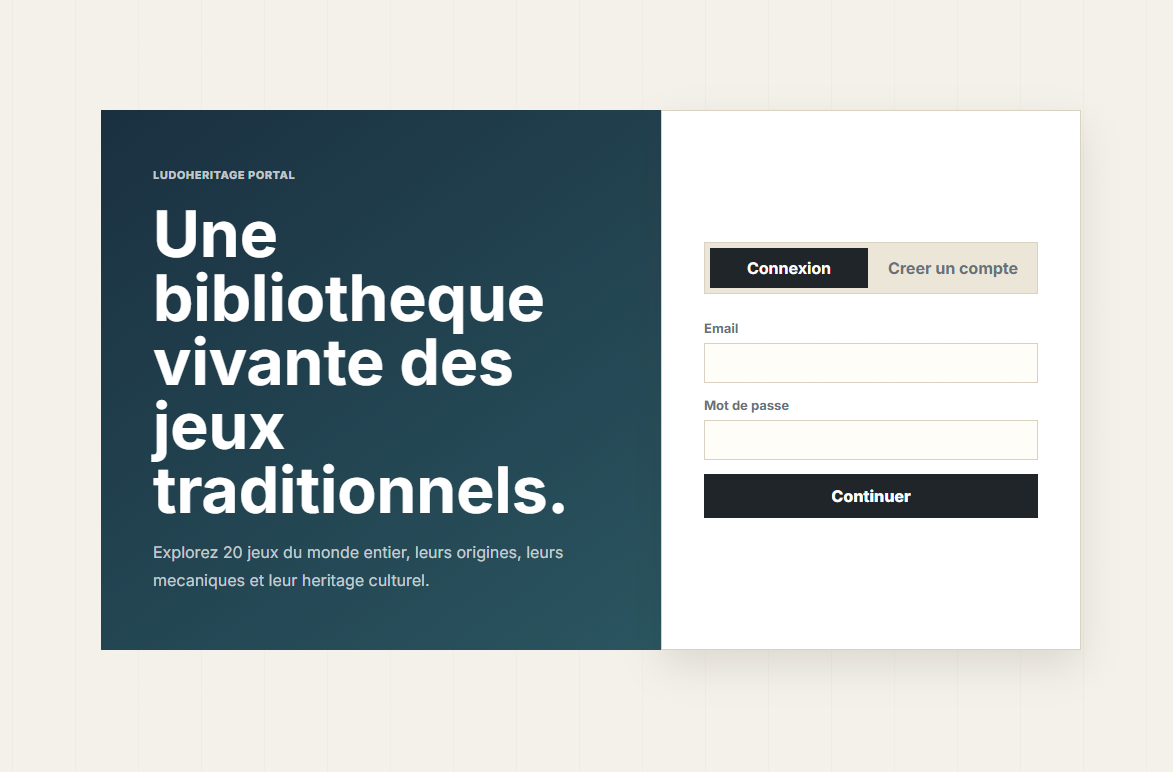
\includegraphics[width=\textwidth]{screenshots/login.png}
        \caption{Page de connexion}
        \label{fig:login}
    \end{subfigure}
    \hfill
    \begin{subfigure}[b]{0.48\textwidth}
        \centering
        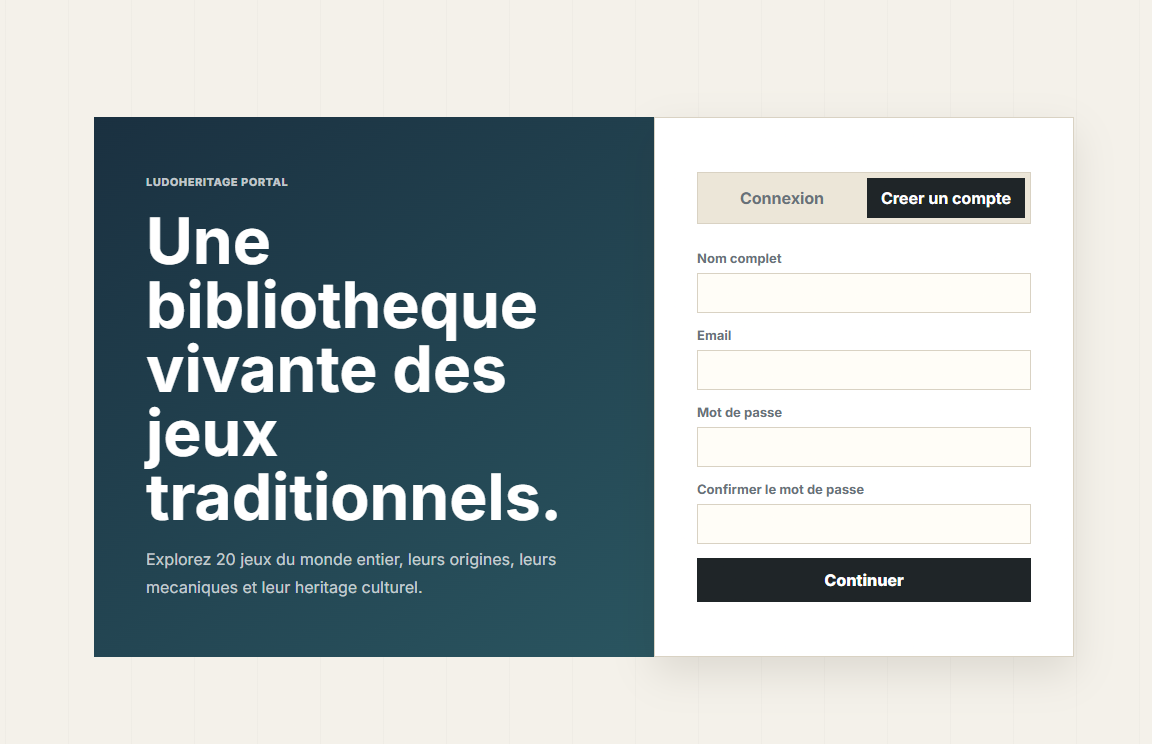
\includegraphics[width=\textwidth]{screenshots/signup.png}
        \caption{Formulaire d'inscription}
        \label{fig:signup}
    \end{subfigure}
    \caption{Interfaces d'authentification de LudoHeritage}
    \label{fig:auth-pages}
\end{figure}

La page d'authentification présente une interface épurée en deux colonnes~: un panneau de gauche
à fond sombre qui introduit la plateforme, et un panneau de droite avec le formulaire. Le formulaire
d'inscription inclut~:

\begin{itemize}
    \item Un champ de nom complet (minimum 2 caractères).
    \item Un champ e-mail validé côté backend (annotation \texttt{@Email}).
    \item Un mot de passe et sa confirmation, avec vérification de correspondance avant l'envoi.
\end{itemize}

Côté backend, le mot de passe est hashé avec \textbf{BCrypt} avant stockage. En cas d'erreur
(e-mail déjà existant, données invalides), le gestionnaire global \texttt{GlobalExceptionHandler}
retourne un message d'erreur lisible directement affiché à l'utilisateur.

\subsection{Questionnaire d'intégration (Onboarding)}

Après la première connexion, l'utilisateur est guidé à travers un questionnaire de quatre
questions pour personnaliser son expérience~:

\begin{itemize}
    \item \textbf{Niveau de jeu}~: Débutant, Amateur ou Passionné.
    \item \textbf{Type de jeu préféré}~: Stratégie, Hasard, Hasard et stratégie, ou Adresse.
    \item \textbf{Région à explorer}~: Afrique, Asie, Europe ou Amérique.
    \item \textbf{Langue de discussion}~: Français, English ou Arabic.
\end{itemize}

Ces préférences alimentent les recommandations de LudoBot et les jeux suggérés dans le profil.

% ─────────────────────────────────────────────────────────────────────────────
\section{Catalogue des jeux}
% ─────────────────────────────────────────────────────────────────────────────

\subsection{Vue d'ensemble}

Le catalogue est le cœur de LudoHeritage. Il recense vingt jeux traditionnels, chacun représenté
par une carte synthétique affichant~: la période, le statut de reconstruction, le nom, le pays
d'origine, les catégories de mécanique, le nombre de joueurs, et un indicateur de favori.

\begin{figure}[H]
    \centering
    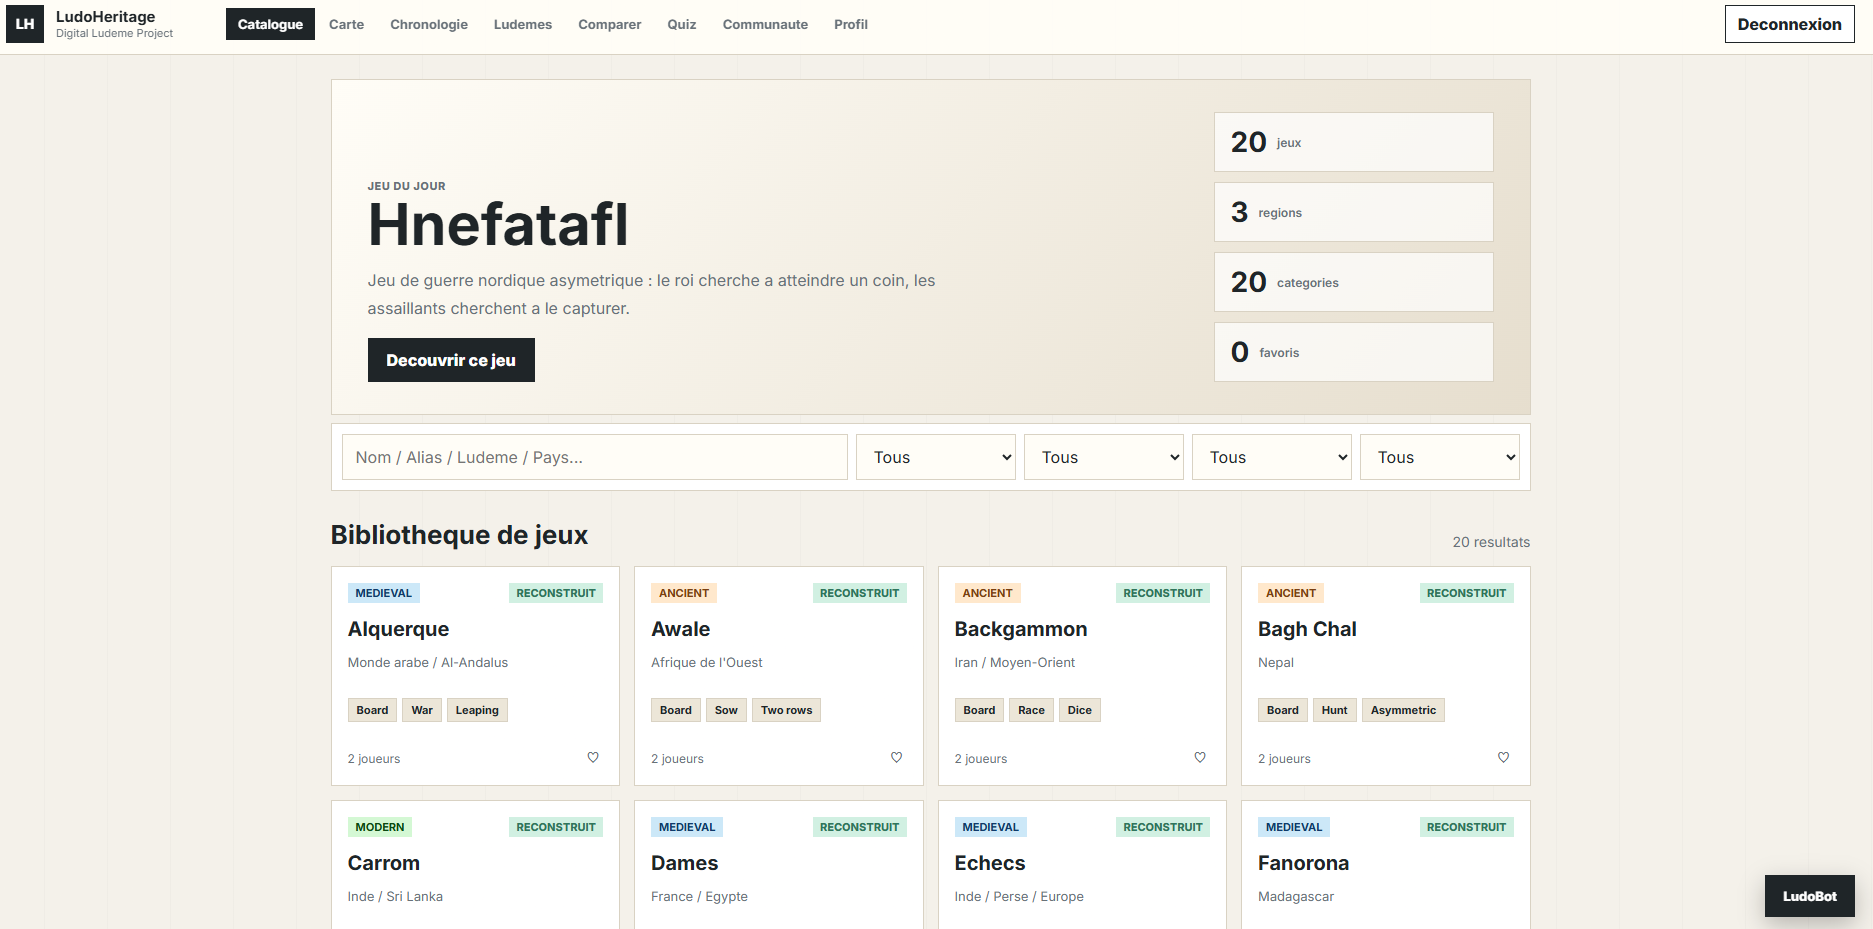
\includegraphics[width=0.95\textwidth]{screenshots/catalogue.png}
    \caption{Catalogue des jeux -- Filtrage par région, période et niveau}
    \label{fig:catalogue}
\end{figure}

La barre de filtres permet de restreindre l'affichage selon cinq critères cumulables~:
une \textbf{recherche textuelle} (nom, alias, pays, mécanique), la \textbf{période}
(Ancien, Médiéval, Moderne), la \textbf{région} (Afrique, Asie, Europe, Amérique),
la \textbf{catégorie} et le \textbf{niveau} recommandé.

\subsection{Fiche détaillée d'un jeu}

Au clic sur une carte, une fenêtre modale s'ouvre avec quatre onglets~:

\begin{enumerate}
    \item \textbf{Aperçu}~: description synthétique, faits rapides (pays, période, joueurs, durée).
    \item \textbf{Règles}~: explication complète des règles + tutoriel visuel pas-à-pas
          (plateaux Avant/Après pour chaque mouvement).
    \item \textbf{Histoire}~: contexte historique et culturel du jeu, avec références documentaires.
    \item \textbf{Mécanique}~: résumé des ludèmes (mécaniques de jeu) et catégories.
\end{enumerate}

Pour les jeux jouables en ligne (Awale), un cinquième onglet \og{}\textbf{Jouer ▶}\fg{} permet
de lancer directement une partie dans le navigateur.

% ─────────────────────────────────────────────────────────────────────────────
\section{Carte mondiale interactive}
% ─────────────────────────────────────────────────────────────────────────────

La page \textbf{Carte} offre une visualisation géographique de la distribution des jeux dans
le monde. Une carte SVG interactive représente les continents, et chaque jeu apparaît sous
forme d'un point blanc positionné sur sa région d'origine.

\begin{figure}[H]
    \centering
    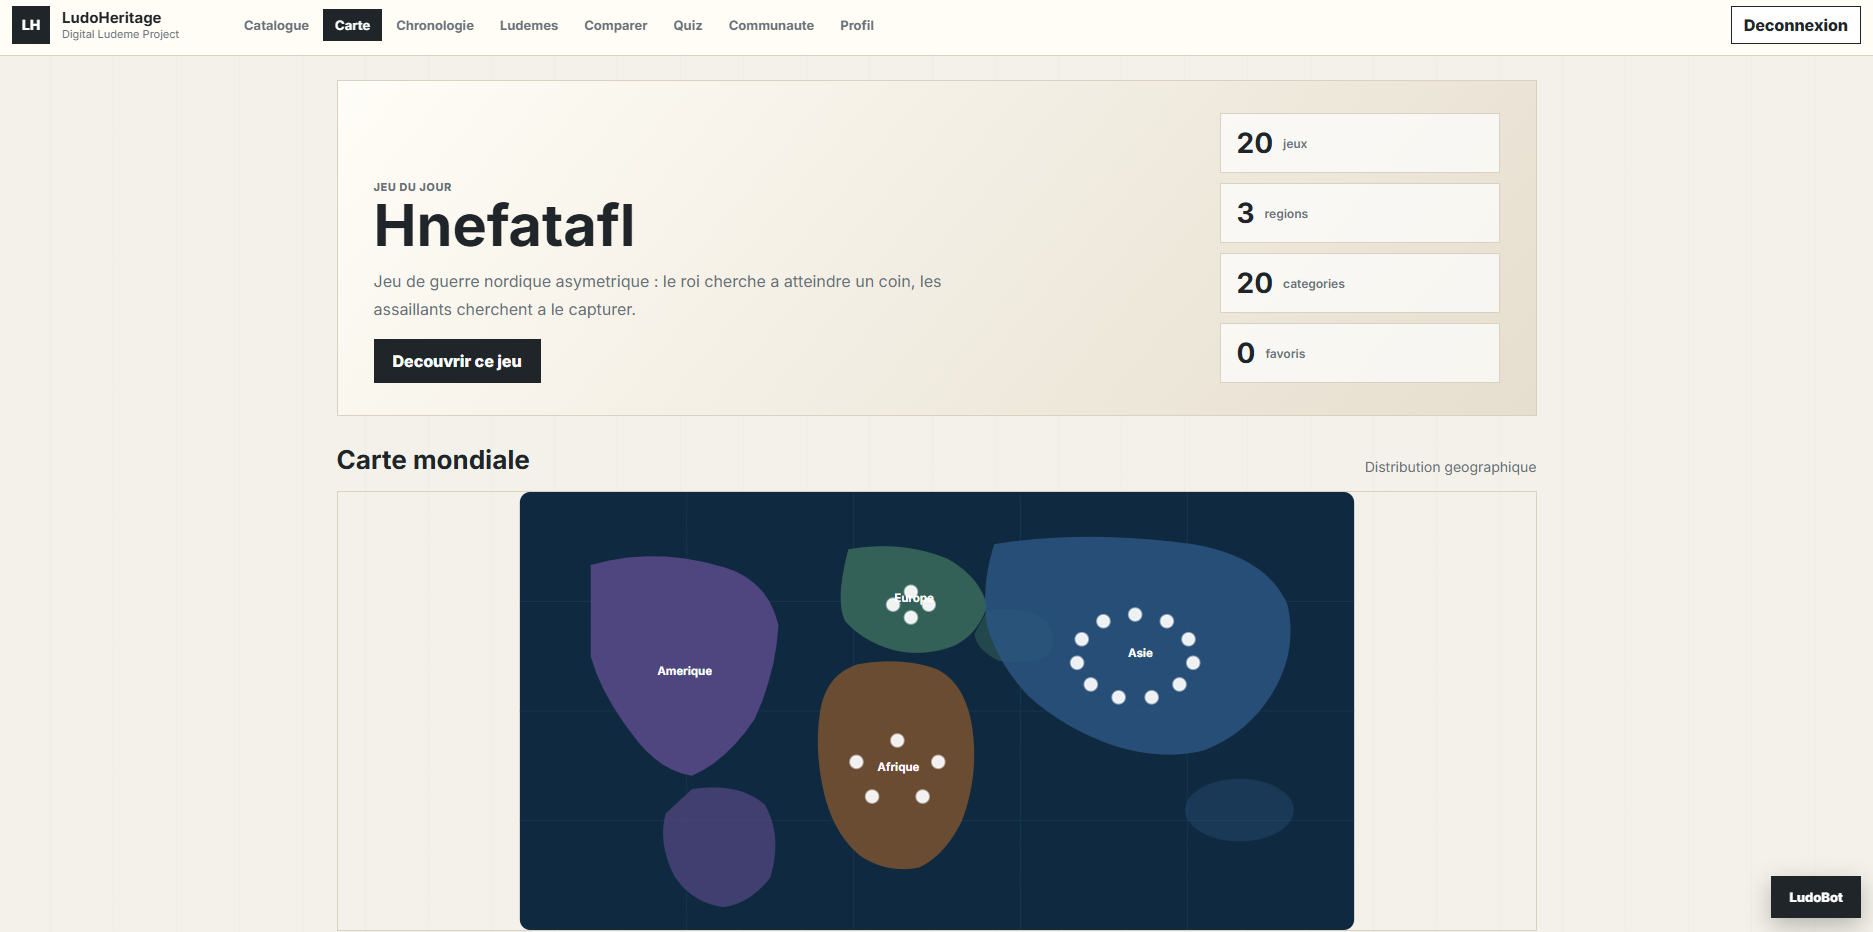
\includegraphics[width=0.95\textwidth]{screenshots/carte.png}
    \caption{Carte mondiale -- Distribution géographique des 20 jeux}
    \label{fig:carte}
\end{figure}

L'utilisateur peut~:
\begin{itemize}
    \item \textbf{Cliquer sur un continent} pour filtrer le catalogue sur cette région.
    \item \textbf{Survoler un point blanc} pour voir le nom du jeu correspondant.
    \item \textbf{Cliquer sur un point} pour ouvrir directement la fiche du jeu.
\end{itemize}

Des cartes régionales au bas de la page affichent le nom de la région, le nombre de jeux
documentés et les premiers noms de jeux pour faciliter la navigation.

% ─────────────────────────────────────────────────────────────────────────────
\section{Chronologie historique}
% ─────────────────────────────────────────────────────────────────────────────

La \textbf{Chronologie} est l'une des fonctionnalités les plus originales de LudoHeritage. Elle
place les vingt jeux sur une frise temporelle horizontale défilante, ordonnée du jeu le plus
ancien au plus récent.

\begin{figure}[H]
    \centering
    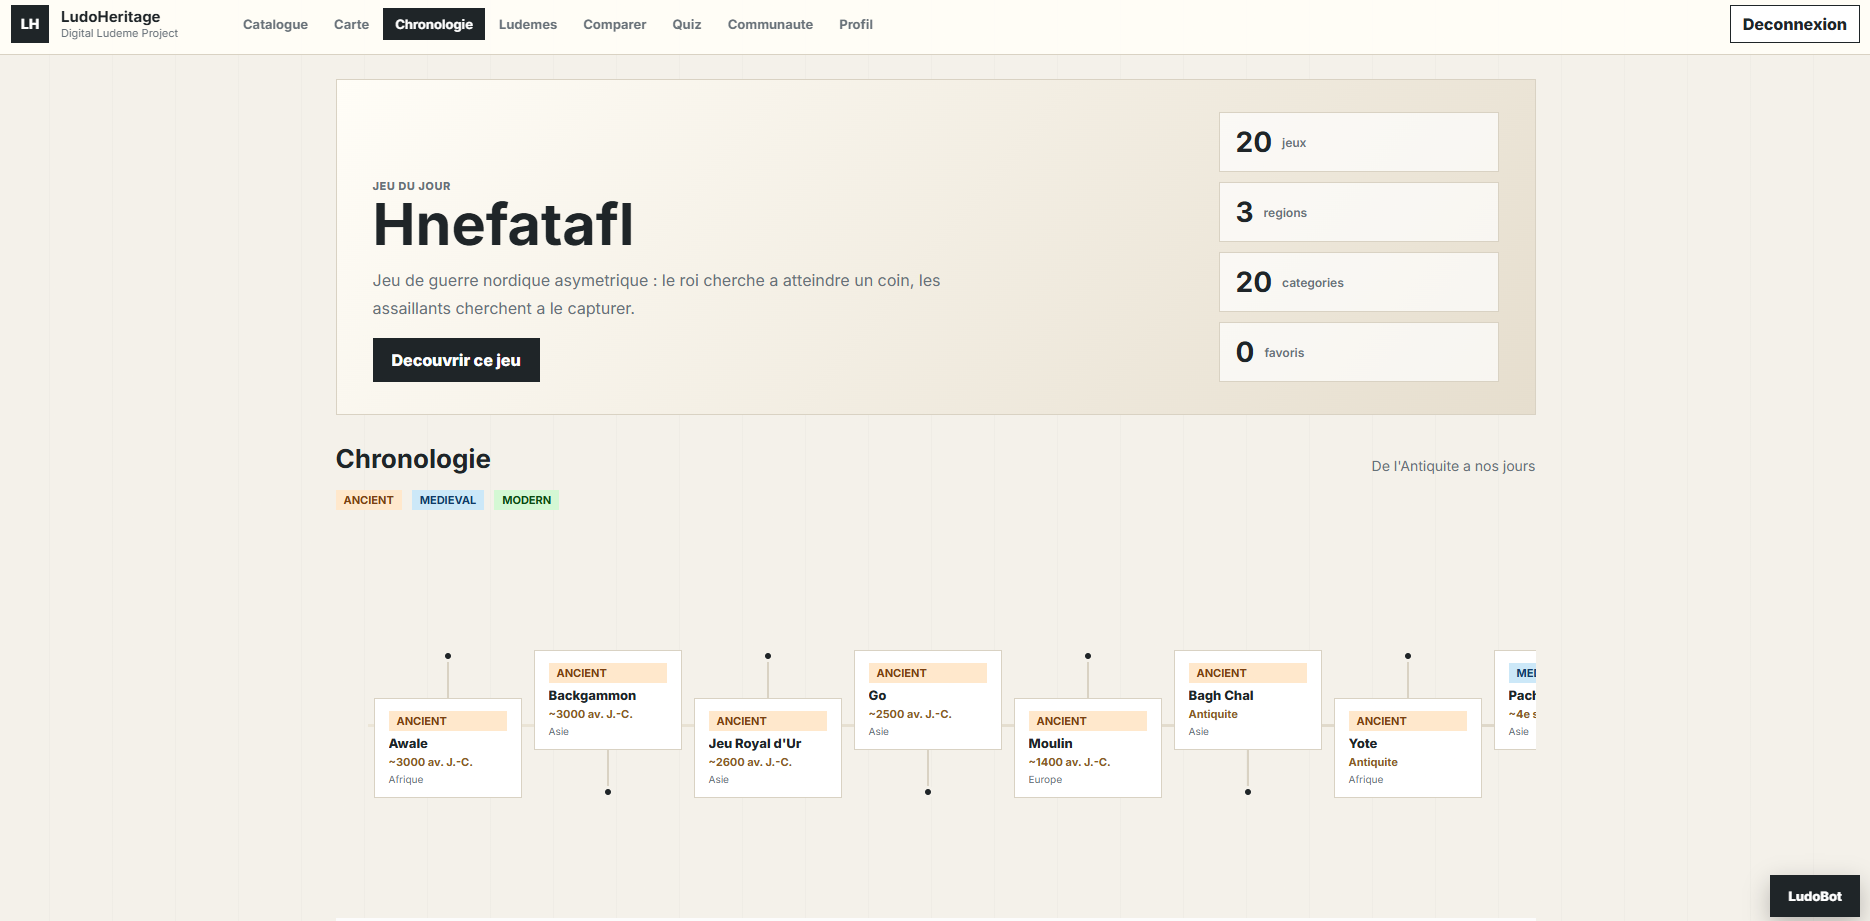
\includegraphics[width=0.95\textwidth]{screenshots/chronologie.png}
    \caption{Chronologie historique -- De l'Antiquité à l'ère moderne}
    \label{fig:chronologie}
\end{figure}

Chaque jeu est représenté par une carte alternant au-dessus et en dessous d'une ligne centrale,
pour éviter les chevauchements. Les cartes sont codées par couleur selon la période~:
\begin{itemize}
    \item \textbf{Orange}~: jeux Anciens (avant 500 ap. J.-C.),
    \item \textbf{Bleu}~: jeux Médiévaux (500 -- 1500 ap. J.-C.),
    \item \textbf{Vert}~: jeux Modernes (après 1500 ap. J.-C.).
\end{itemize}

Cette visualisation illustre à la fois l'ancienneté du phénomène ludique (certains jeux datent
de 3000 ans avant J.-C.) et sa continuité jusqu'à nos jours.

% ─────────────────────────────────────────────────────────────────────────────
\section{Ludèmes et mécaniques de jeu}
% ─────────────────────────────────────────────────────────────────────────────

Inspirée du système de \textit{ludèmes} du projet Ludii, la page \textbf{Ludèmes} de LudoHeritage
organise les jeux par catégorie de mécanique.

\begin{figure}[H]
    \centering
    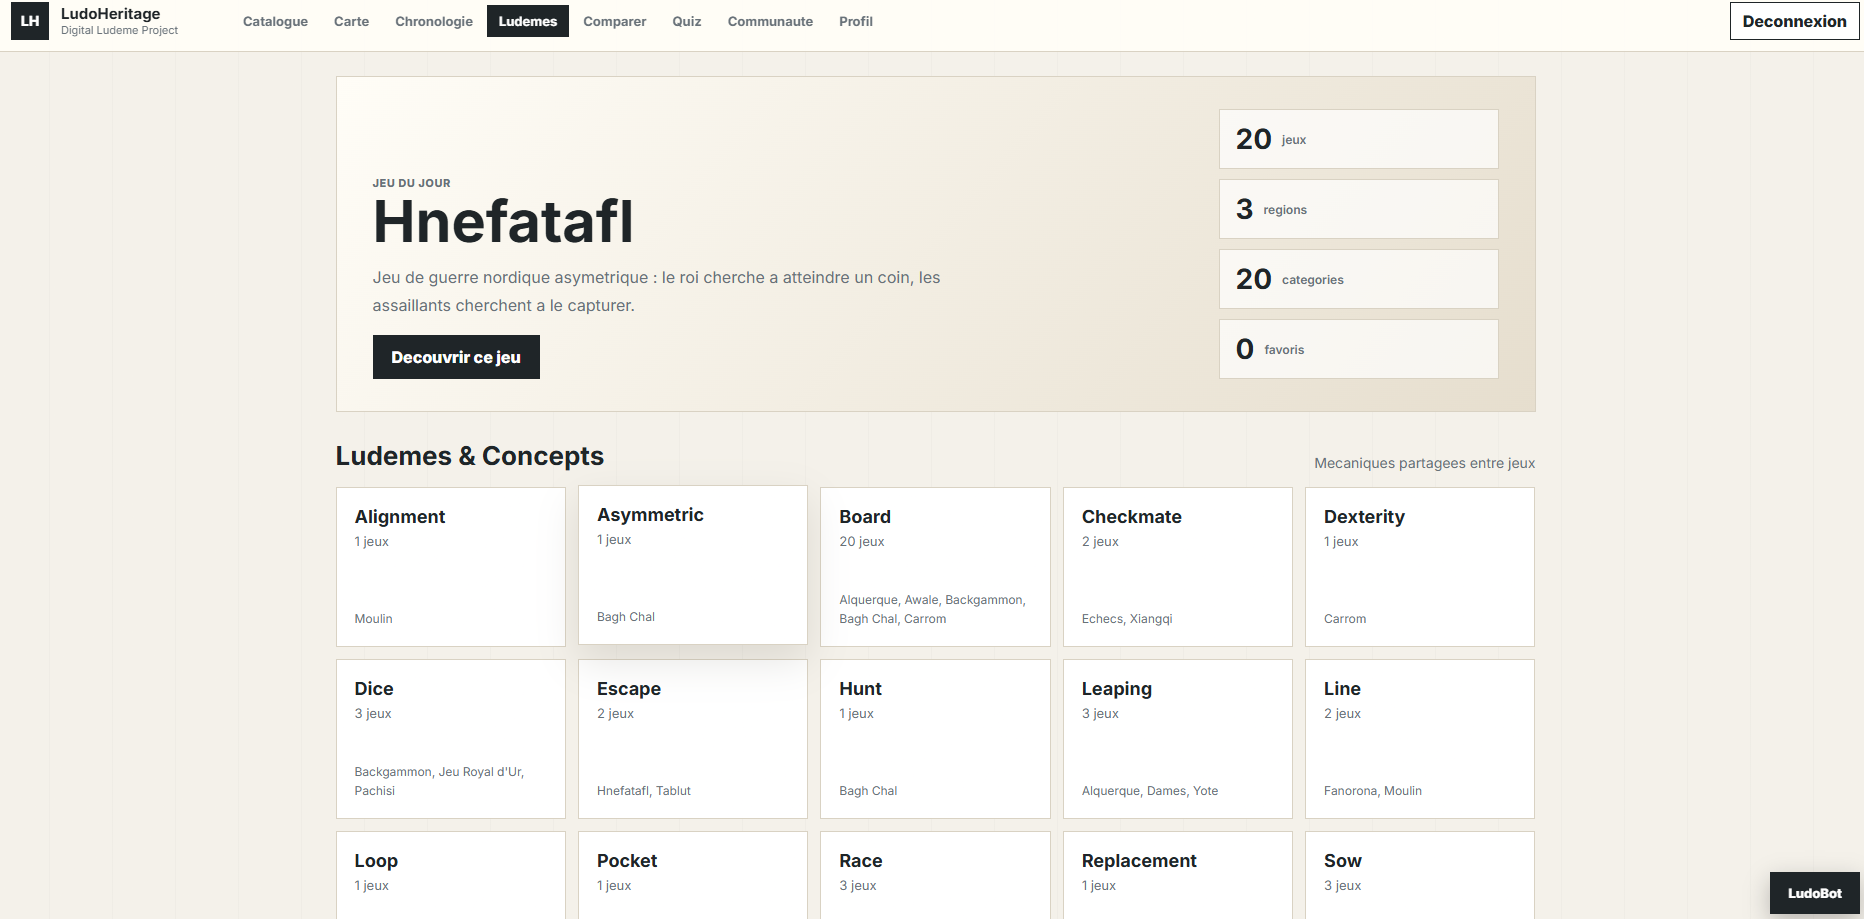
\includegraphics[width=0.95\textwidth]{screenshots/ludemes.png}
    \caption{Page des Ludèmes -- Mécaniques partagées entre jeux}
    \label{fig:ludemes}
\end{figure}

Chaque carte de catégorie indique le nombre de jeux qui partagent cette mécanique et les liste.
Un clic sur une catégorie filtre automatiquement le catalogue. Cette fonctionnalité permet aux
utilisateurs de~:
\begin{itemize}
    \item Comprendre les familles de jeux (ex.~: tous les jeux de semailles).
    \item Trouver des jeux similaires à un jeu qu'ils connaissent déjà.
    \item Explorer des mécaniques transculturelles (ex.~: la capture par saut existe en Afrique,
          en Europe et en Asie).
\end{itemize}

% ─────────────────────────────────────────────────────────────────────────────
\section{Outil de comparaison}
% ─────────────────────────────────────────────────────────────────────────────

L'outil \textbf{Comparer} permet de placer deux jeux côte à côte pour une analyse comparative
détaillée.

\begin{figure}[H]
    \centering
    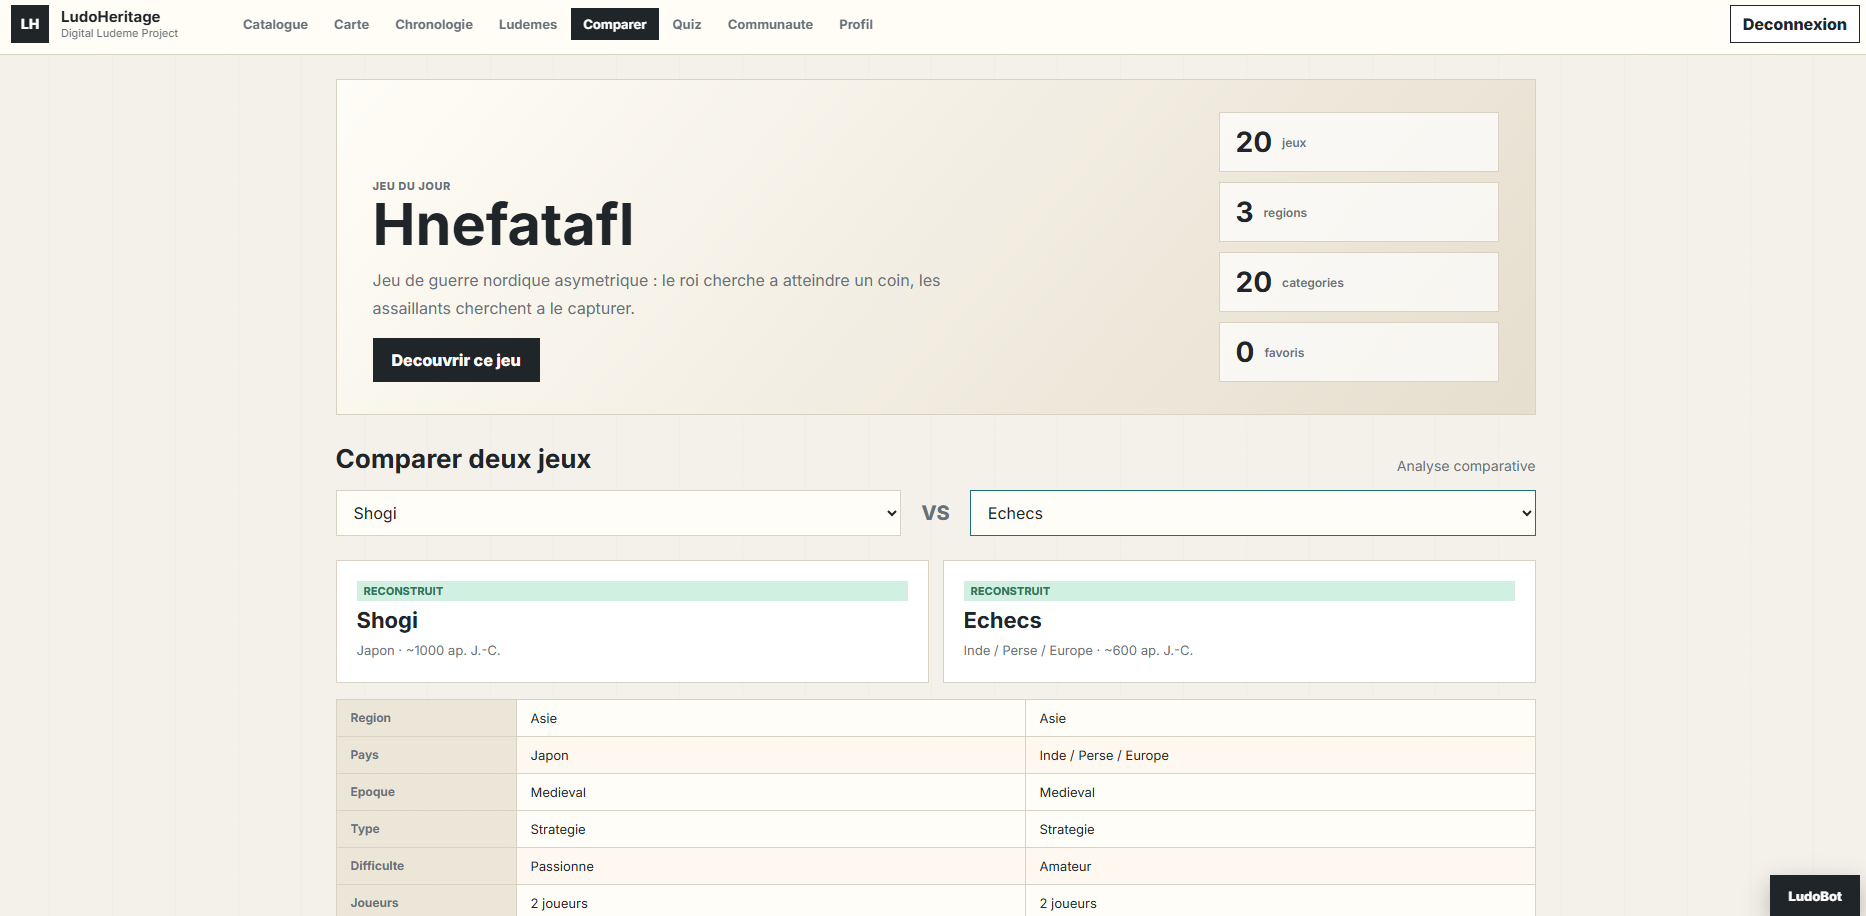
\includegraphics[width=0.95\textwidth]{screenshots/comparaison.png}
    \caption{Outil de comparaison -- Analyse côte à côte de deux jeux}
    \label{fig:comparaison}
\end{figure}

L'utilisateur sélectionne deux jeux via deux menus déroulants. Le système affiche ensuite~:

\begin{itemize}
    \item Une \textbf{table de comparaison} sur onze critères (région, pays, époque, type,
          difficulté, joueurs, durée, etc.) avec mise en évidence des différences en fond orange.
    \item Les \textbf{ludèmes de chaque jeu} avec les mécaniques partagées mis en avant en vert.
    \item Un \textbf{encadré des ludèmes communs} lorsque les deux jeux partagent des mécaniques,
          illustrant les liens transhistoriques entre civilisations.
\end{itemize}

% ─────────────────────────────────────────────────────────────────────────────
\section{Module Quiz et Classement}
% ─────────────────────────────────────────────────────────────────────────────

\begin{figure}[H]
    \centering
    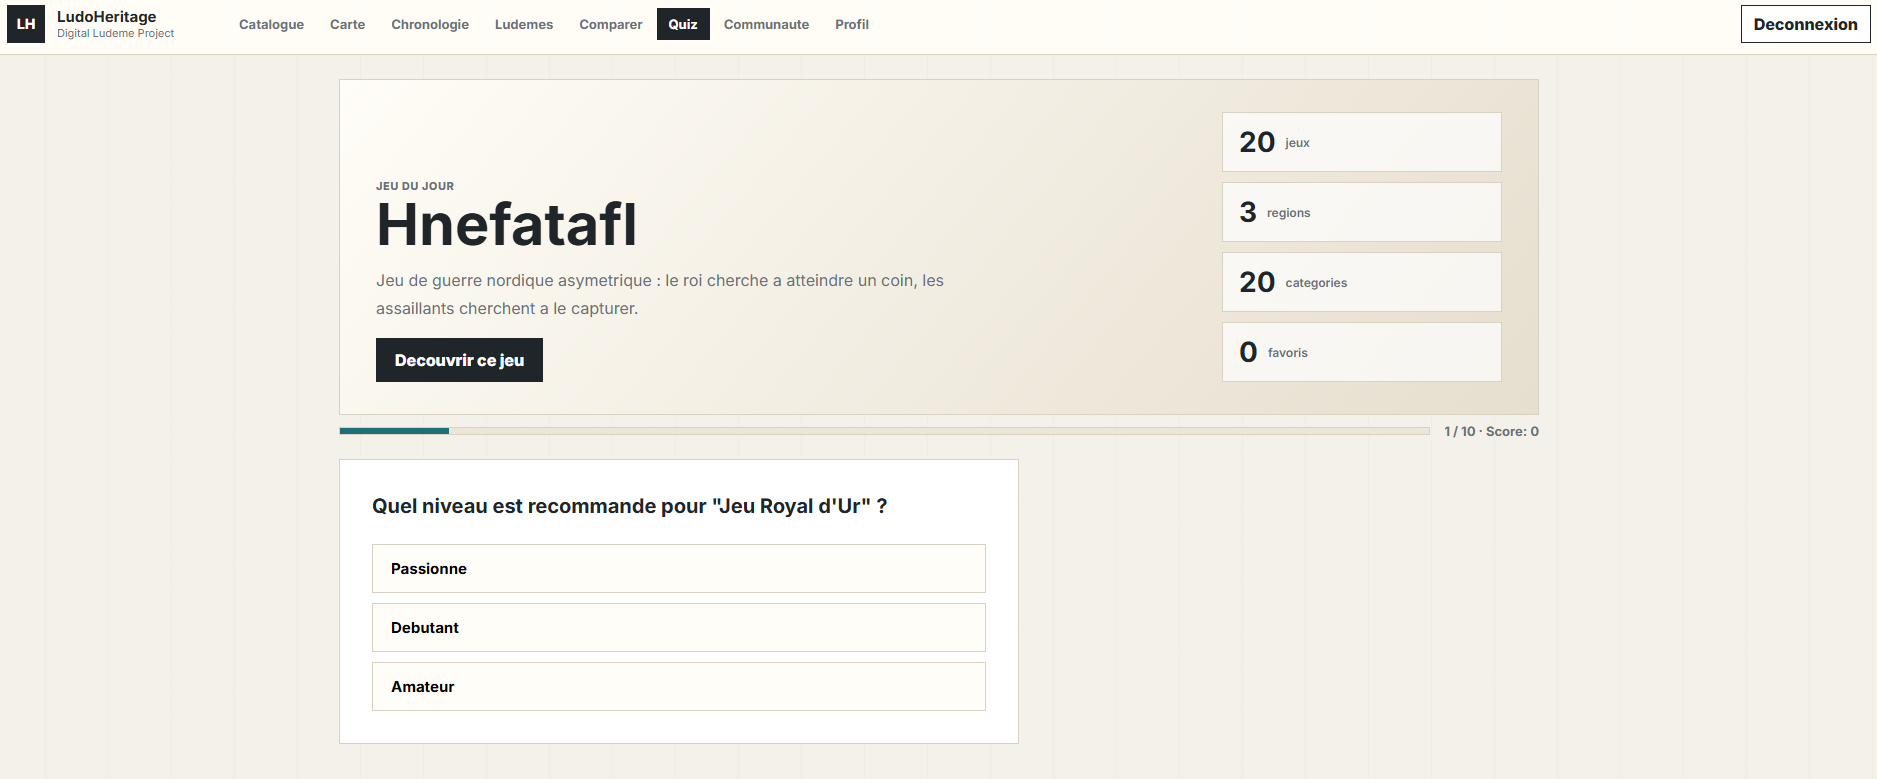
\includegraphics[width=0.95\textwidth]{screenshots/quiz.png}
    \caption{Module Quiz -- Questions interactives avec classement}
    \label{fig:quiz}
\end{figure}

Le module \textbf{Quiz} propose des sessions de dix questions à choix multiples, générées
dynamiquement à partir des données du catalogue. Les questions portent sur~:
la région d'origine d'un jeu, son époque, son type, et son niveau de difficulté recommandé.

À chaque réponse, un retour immédiat est affiché (bonne réponse en vert, mauvaise en rouge).
À la fin de la session, le score est affiché sous forme graphique et soumis automatiquement au
classement mondial via l'API \texttt{POST /api/quiz/scores}. Le classement affiche les dix
meilleurs scores de tous les utilisateurs.

% ─────────────────────────────────────────────────────────────────────────────
\section{Forum communautaire}
% ─────────────────────────────────────────────────────────────────────────────

\begin{figure}[H]
    \centering
    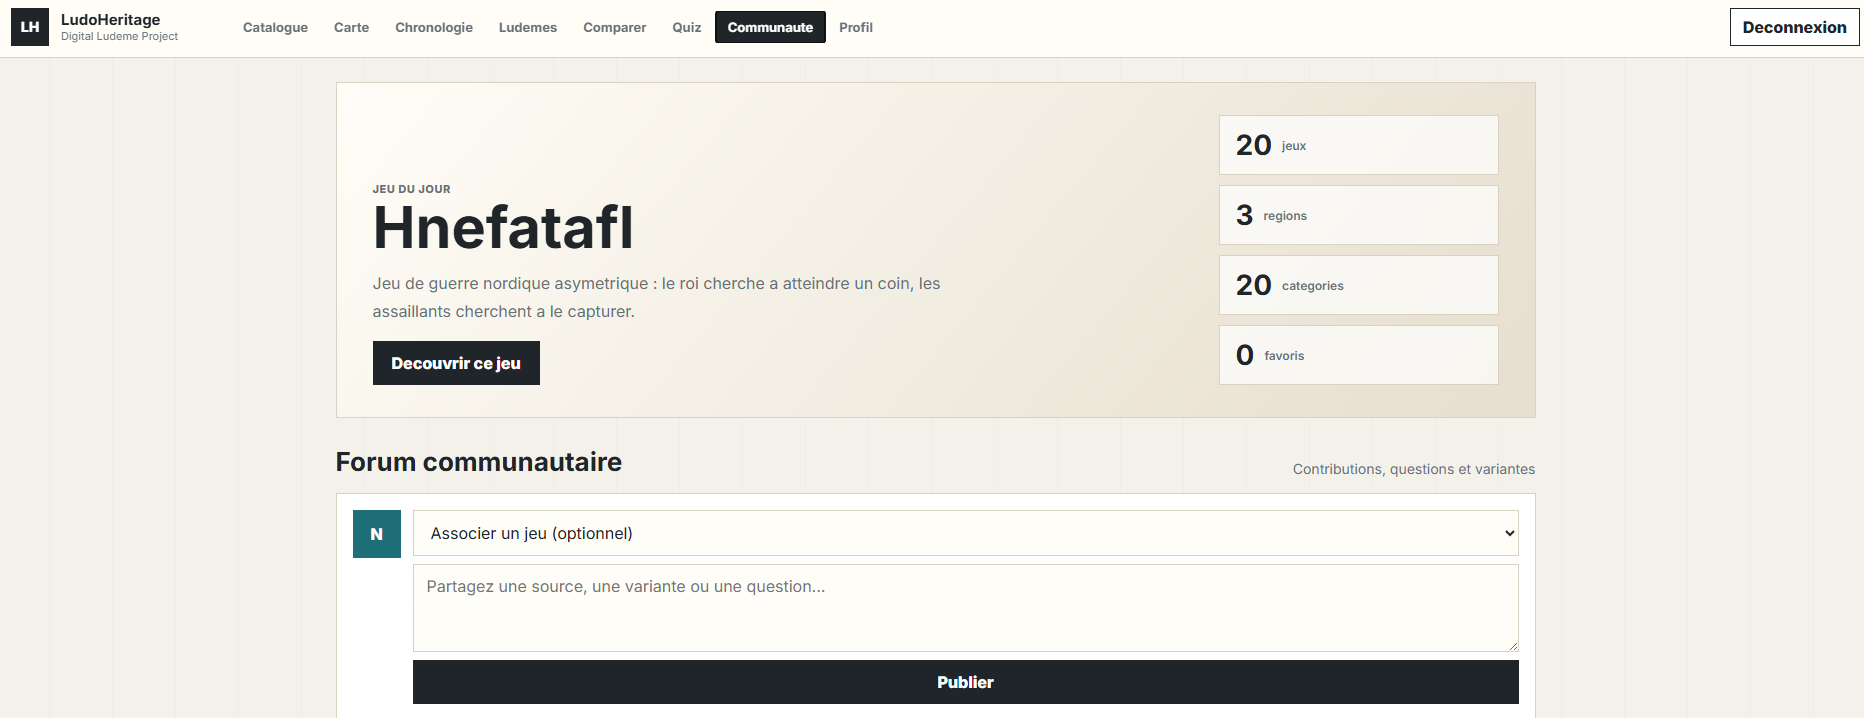
\includegraphics[width=0.95\textwidth]{screenshots/commauntie.png}
    \caption{Forum communautaire -- Publications et échanges entre utilisateurs}
    \label{fig:communaute}
\end{figure}

Le \textbf{Forum communautaire} permet aux utilisateurs de publier des messages, de les lier à
un jeu du catalogue, de recevoir des likes et des commentaires. Chaque publication affiche le
nom de l'auteur, l'heure de publication (relatif), et le jeu associé si applicable. Les données
sont persistées dans MongoDB via l'API \texttt{/api/community}.

% ─────────────────────────────────────────────────────────────────────────────
\section{Profil utilisateur enrichi}
% ─────────────────────────────────────────────────────────────────────────────

\begin{figure}[H]
    \centering
    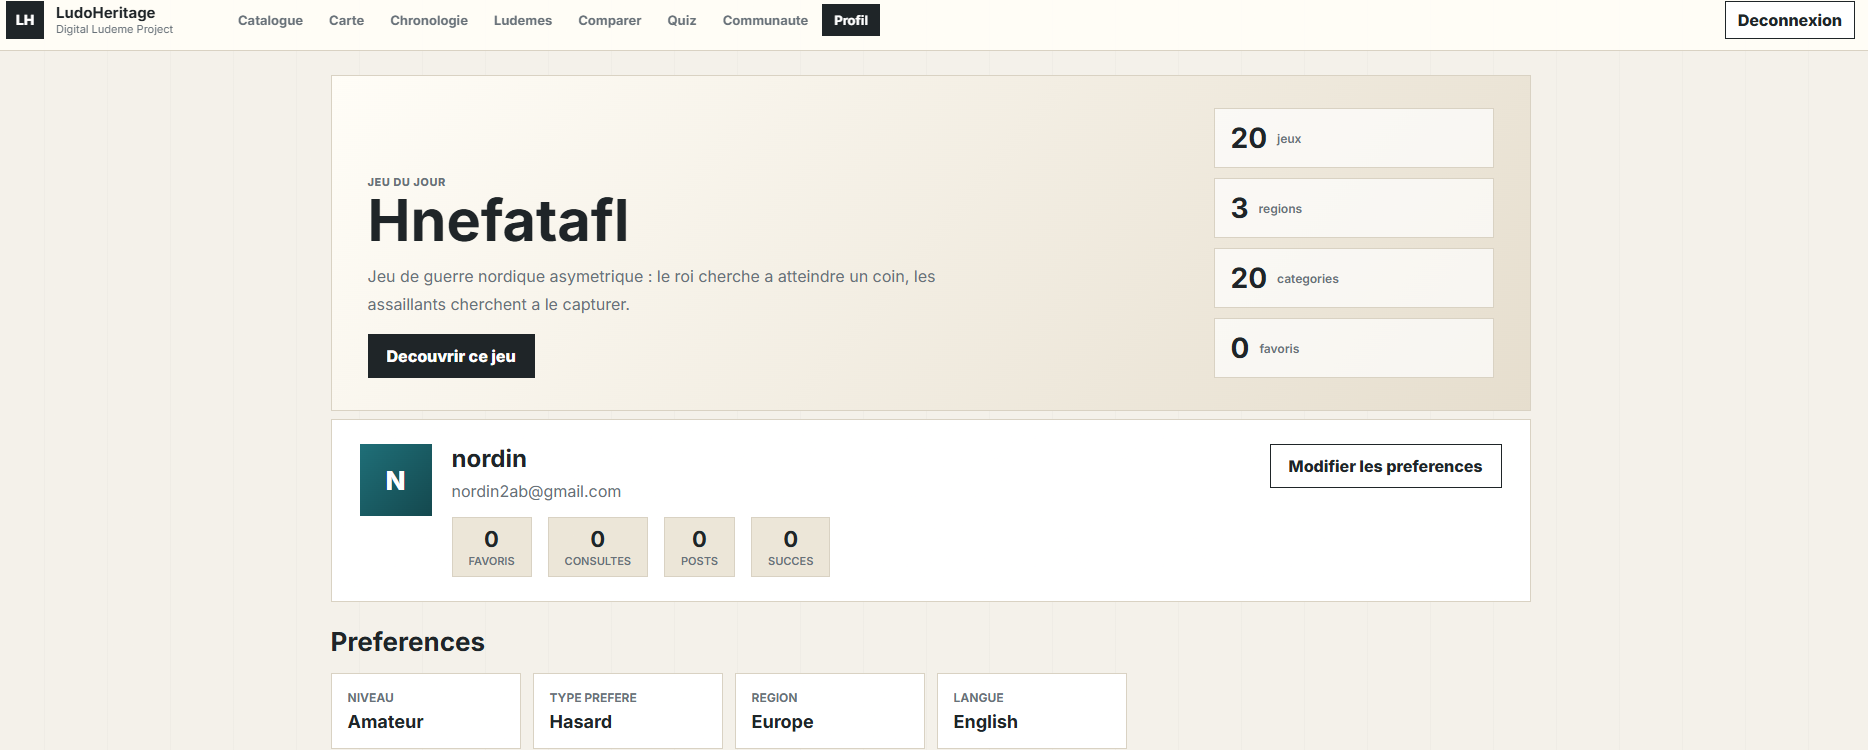
\includegraphics[width=0.95\textwidth]{screenshots/profil.png}
    \caption{Profil utilisateur -- Succès, favoris et recommandations personnalisées}
    \label{fig:profil}
\end{figure}

La page \textbf{Profil} est un tableau de bord personnalisé qui regroupe~:

\begin{itemize}
    \item Un \textbf{en-tête} avec l'avatar, le nom, l'e-mail et quatre compteurs rapides
          (favoris, jeux consultés, posts publiés, succès débloqués).
    \item Un \textbf{éditeur de préférences} inline pour modifier son niveau, son type de jeu
          préféré, sa région et sa langue, sans quitter la page.
    \item Un \textbf{tableau des succès}~: dix badges à débloquer en explorant la plateforme
          (Explorateur, Historien, Collectionneur, Citoyen du monde, etc.).
    \item Une \textbf{liste de recommandations} personnalisées basées sur les préférences.
    \item L'\textbf{historique des jeux récemment consultés}, persisté localement.
    \item Les \textbf{jeux favoris} et les \textbf{publications communautaires} de l'utilisateur.
\end{itemize}

% ─────────────────────────────────────────────────────────────────────────────
\section{LudoBot -- Assistant IA}
% ─────────────────────────────────────────────────────────────────────────────

\textbf{LudoBot} est l'assistant conversationnel de LudoHeritage, accessible depuis un bouton
flottant en bas à droite de toutes les pages. Il repose sur un modèle de langage local
(\textbf{Ollama}) et une couche de traitement intelligente côté backend (\texttt{AgentService}).

\subsection{Fonctionnement technique}

Lorsqu'un utilisateur envoie un message, le \texttt{AgentService} applique les étapes suivantes~:

\begin{enumerate}
    \item \textbf{Détection d'intention}~: identification de l'intention parmi dix catégories
          (recommandation, règles, histoire, comparaison, quiz, stratégie, culture, etc.).
    \item \textbf{Détection de sentiment}~: adaptation du ton de la réponse (positif, négatif,
          confus, neutre).
    \item \textbf{Recherche de jeux pertinents}~: sélection des jeux du catalogue correspondant
          au contexte de la question.
    \item \textbf{Construction du prompt}~: assemblage d'un prompt système personnalisé + le
          contexte des jeux + le message de l'utilisateur.
    \item \textbf{Appel à Ollama}~: envoi du prompt au modèle via \texttt{OllamaChatClient}
          (API \texttt{/api/generate}).
    \item \textbf{Réponse de secours}~: si Ollama est hors ligne, une réponse pertinente est
          générée sans LLM à partir du contexte des jeux.
\end{enumerate}

Le panneau du chat affiche en temps réel le statut d'Ollama (connecté avec le nom du modèle,
ou hors ligne) dès l'ouverture.

% ─────────────────────────────────────────────────────────────────────────────
\section{Jeu jouable -- Awale}
% ─────────────────────────────────────────────────────────────────────────────

LudoHeritage intègre une version jouable de l'\textbf{Awale} directement dans le navigateur,
accessible depuis l'onglet \og{}Jouer ▶\fg{} de la fiche du jeu.

L'implémentation respecte les règles traditionnelles~: douze cases disposées en deux rangées de
six, semailles dans le sens anti-horaire, capture par la règle des 2-3 graines. Le jeu est
conçu pour deux joueurs en local (\textit{pass-and-play}).

La décision de ne rendre jouable que l'Awale (et non les 19 autres jeux) est intentionnelle~:
des jeux comme les Échecs, le Go ou le Shogi nécessitent des interfaces visuelles élaborées
et des moteurs de jeu complexes qui dépassent le cadre de ce projet. L'Awale, avec son plateau
de cases numérotées, se prête naturellement à une représentation simplifiée.

% ─────────────────────────────────────────────────────────────────────────────
\section{Conclusion}
% ─────────────────────────────────────────────────────────────────────────────

Ce chapitre a présenté l'ensemble des fonctionnalités de LudoHeritage, illustrées par des
captures d'écran de l'application. La plateforme offre une expérience complète et cohérente,
allant de la simple consultation du catalogue à l'interaction avec un assistant IA, en passant
par la visualisation géographique, le quiz et la participation communautaire. Le prochain
chapitre présente les tests effectués pour valider le bon fonctionnement de l'application.
